\section{Diseño}
    
    Se presenta el equipo utilizado, como se distribuye fisicamente sobre
    el piso de la oficina, y como se distribuye el cableado en cada
    sección; la configuración (y estructura) lógica de la red, y los
    servicios que esta ofrece.

    \subsection{Lista de equipo}
        % Tablas c/u, enfoque en listado
        
        Se presenta únicamente el equipo utilizado (no la cantidad),
        así como el precio de cada unidad y el proveedor del mismo.
        Se discute brevemente el rol de cada uno en el diseño completo. 

        \subsubsection{Electrónica de Red}
            
            En la tabla \ref{tab: ElectronicaRed} se presenta el equipo
            electrónico presente en la red. Se construye una única red
            de capa 3, que trabaje sobre las redes virtuales de area 
            local definidas, utilizando los servidores para asignación
            dinámica de direcciónes IP de usuarios (fijos e 
            inalámbricos).
            

            % =========================================================
            %  Commands for the table, for more organized structure
            % =========================================================
            \newcommand{\ColumnQuantity}{4}
            \newcommand{\f}{\footnotesize}
            \newcommand{\Router}{https://www.router-switch.com/cisco-isr4331-k9-p-16544.html}
            \newcommand{\Switch}{https://www.router-switch.com/ws-c2960-24tc-s-p-5255.html}
            \newcommand{\AccessPoint}{https://www.amazon.com/TP-Link-EAP610-Business-Wireless-Integrated/dp/B09G5H4XS2?th=1}
            \newcommand{\APsheet}{https://www.tp-link.com/baltic/business-networking/omada-sdn-access-point/eap610/#specifications}
            \newcommand{\Server}{https://www.theserverstore.com/cisco-ucs-c220-m5-10-bay-1u-rackmount-server.html}
            \newcommand{\ServerDatasheet}{https://www.cisco.com/c/en/us/products/collateral/servers-unified-computing/ucs-c-series-rack-servers/datasheet-c78-739281.html}

            % =========================================================
            %  Table
            % =========================================================

            \begin{xltabular}{\linewidth}{|>{\f}X|>{\f}X|>{\f}X|>{\f}X|}
                \caption{Lista de tipos de electrónica de red utilizada}
                \label{tab: ElectronicaRed}                                  
                %\addtocounter{table}{-1} \\
                \hline
                \textbf{Equipo} & \textbf{Proveedor} & \textbf{Precio Unitario} & \textbf{Descripción} \\   
                \hline 
                \endfirsthead
                \caption[]{Description of Variables used in this Study (Cont.)} \\
                \hline
                \textbf{Equipo} & \textbf{Proveedor} & \textbf{Precio Unitario} & \textbf{Descripción} \\   
                \hline
                \endhead
                \multicolumn{\ColumnQuantity}{r}{\footnotesize\textit{Continue on the next page}}
                \endfoot
                \hline
                \endlastfoot
                
                ISR4331         & \href{\Router}{Cisco}         &  \$1,066.00      & Router, establece la capa 3 completa del edificio. \\  \hline
                WS-C2960+24TC-S & \href{\Switch}{Cisco}         &  \$472.00        & Switch, define las VLANs privada, pública, y acceso a estas. \\  \hline
                EAP610          & \href{{\AccessPoint}}{TPLink} &  \$80.99         & Punto de acceso inalámbrico utilizado en la red (\href{\APsheet}{Caracteristicas}). \\  \hline
                UCS C220 M5     & \href{\Server}{Cisco}         &  \$773.00/735.00 & Servidor con/sin tarjetas de red (\href{\ServerDatasheet}{características}). \\  \hline
                
            \end{xltabular}
                

        \subsubsection{Cableado Estructurado}

            En la tabla \ref{tab: CableadoEstructurado} se presentan
            los materiales utilizados en la canalización de la red, 
            así como los tipos de cables a utilizar por el equipo
            electrónico durante el funcionamiento de la red. Se incluye
            una descripción de la función que tiene y el lugar fisico
            de cada uno de los componentes mencionados.

            % =========================================================
            %  Commands for the table, for more organized structure
            % =========================================================
            
            \newcommand{\Canaleta}{https://cr.epaenlinea.com/canaleta-de-200-x-10-x-5-cm-color-blanco.html}
            \newcommand{\Canastas}{https://www.iesacr.com/shop/ba7248-canasta-electrozinc-100x65x3000mm-basor-bf2r100x65-11072?category=477#attr=}
            \newcommand{\EthernetCable}{https://www.amazon.com/Amazon-Basics-Ethernet-Gold-Plated-Connectors/dp/B00N2VIALK?th=1}
            \newcommand{\Extenciones}{https://cr.epaenlinea.com/extension-electrica-16-awg-3-m-uso-pesado-naranja.html}

            % =========================================================
            %  Table
            % =========================================================

            \begin{xltabular}{\linewidth}{|>{\f}X|>{\f}X|>{\f}X|>{\f}X|}
                \caption{Lista de materiales para la canalización de la red}
                \label{tab: CableadoEstructurado}                                  
                %\addtocounter{table}{-1} \\
                \hline
                \textbf{Equipo} & \textbf{Proveedor} & \textbf{Precio Unitario} & \textbf{Descripción} \\   
                \hline 
                \endfirsthead
                \caption[]{Description of Variables used in this Study (Cont.)} \\
                \hline
                \textbf{Equipo} & \textbf{Proveedor} & \textbf{Precio Unitario} & \textbf{Descripción} \\   
                \hline
                \endhead
                \multicolumn{\ColumnQuantity}{r}{\footnotesize\textit{Continue on the next page}}
                \endfoot
                \hline
                \endlastfoot
                
                RJ-45                             & \href{\EthernetCable}{Amazon} & \$4.99/6.99/8.54 & Para conexiónes entre dispositivos electrónicos de red. \\ \hline
                Extensión eléctrica 16 AWG        & \href{\Extenciones}{EPA}      & \$5.96           & Para alimentación de equipo eléctrico asignado a UPS. \\  \hline
                CANASTA ELECTROZINC 100x65x3000mm & \href{\Canastas}{IESA}        & \$16.95          & Para guia de cableado sobre el techo. \\  \hline
                Canaleta de 200 x 10 x 5 cm       & \href{\Canaleta}{EPA}         & \$16.31          & Para cables que bajan del techo o atraviezan el piso. \\  \hline
                
            \end{xltabular}

        \subsubsection{Sistemas de Alimentación Eléctrica} \label{sec: SistemasAlimentacionEnergia}

           La alimentación del equipo nesesario y suficiente para
           mantener funcional la infraestructura de la red se
           encuentra conectada a un espaldo de batería y 
           protector contra sobretensiones UPS, que funciona
           como fuente de alimentación de respaldo de 600VA/300
           vatios. El número de parte es BE600M1 y esta fuente
           cuenta con puerto de carga USB. 
           
           Esta \href{https://www.amazon.com/APC-Battery-Protector-Back-UPS-BE600M1/dp/B01FWAZEIU?th=1}{unidad}
           posee un coste de \$85.49, cuyo proveedor es {\it American Power Conversion}.

        \subsubsection{Sistemas de Seguridad}
            
            \begin{itemize}
                \item {\bf Alimentación y Energía}: Protecciónes
                    contra picos de corriente, apagones, y variaciónes
                    significativas de la calidad eléctrica, se
                    encuentran cubiertas en 
                    \ref{sec: SistemasAlimentacionEnergia}
                \item {\bf Seguridad Lógica}: La separación de la red
                    en {\it redes de area local virtual} para los 
                        usuarios internos y visitantes genera una
                        capa de obstrucción al acceso de los
                        dispositivos finales internos.
                \item {\bf Seguridad Física}: El único acceso que
                    se puede tener a los dispositivos de la red
                    (mencionados en la tabla \ref{tab: ElectronicaRed})
                    es con autorización previa a los gabinetes
                    de los dispositivos. El único acceso que se
                    puede tener a los puertos de los switches
                    es por medio de un cable RJ-45 anteriormente
                    instalado o un punto de acceso de WIFI.
                
            \end{itemize}

    \subsection{Distribución de equipo de red}
        % Conexiónes fisicas para cada parte, montaje, etc
        % Plano y demás
        
        En la figura \ref{fig: plano} se muestra una versión en
        pdf del plano del piso de oficina, con las conexiónes de
        cableado estructurado, y el equipo electrónico en sus 
        lugares respectivos.
    
        \begin{figure}[H]
            \centering
            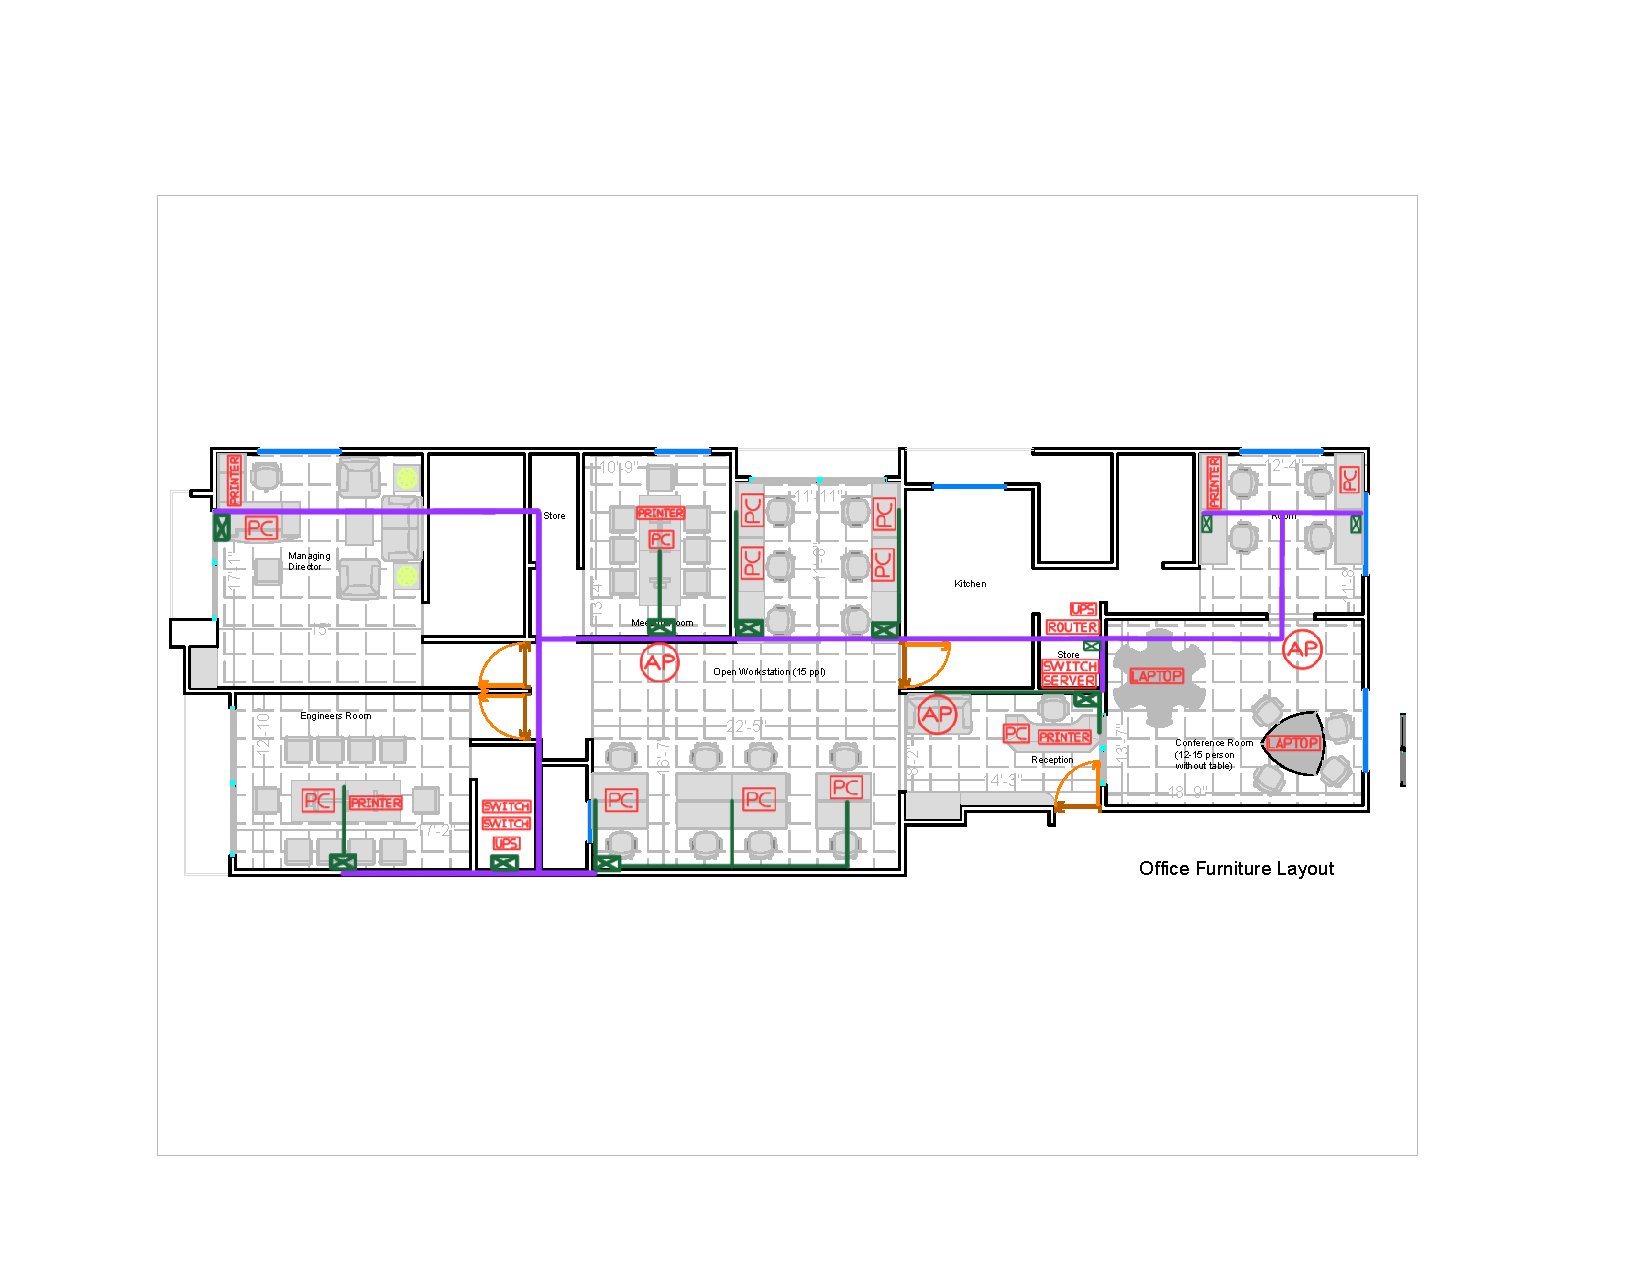
\includegraphics[clip, trim=3cm 6cm 4cm 7cm, width=\linewidth]{figures/PlanoEditado.pdf}
            \caption{Plano Editado con todas las partes}
            \label{fig: plano}
        \end{figure}

        Se mantiene el siguiente código de colores a través de
        este archivo y el \verb|PlanoOficinaFinal.dwg| adjunto:

        \begin{itemize}
            \item Morado: Canastas donde se colocan los cables de
                conexión electrica, así como los RJ-45. Las canastas
                son colocadas sobre el techo de la oficina.
            \item Verde: Las canaletas que bajan los cables de
                las canastas arriba del techo al piso, y llevan
                los cables a través del piso de ser nesesario.
                Los cuadros con una X en medio hacen referencia a
                la canaleta bajando los cables, y las lineas verdes
                horizontales o verticales hacen referencia al
                canalizado a través del piso. 
            \item Rojo: Define el equipo utilizado, en el cuarto
                de ingeniería, asi como en el {\it Store} que se
                encuentra en la cocina, se encuentra las UPS,
                Switches, Routers, y Servidores. Los puntos de
                acceso inalámbrico se encuentran encerrados en
                circulos de color rojo en la zona de trabajo, 
                de conferencias, y recepción. Cabe mencionar que
                se colocaron PC's, impresoras, y Laptops para
                ejemplificar todos los lugares en los que se 
                puede colocar dichos dispositivos.
        \end{itemize}

    \subsection{Estructura Lógica de la Red}
       
        El diseño lógico de la red se separa en la capa 2,
        capa 3, y servicios que ofrece la red.

        \subsubsection{VLANs}

            Se definen tres Switches, de los cuales se sub-dividen
            únicamente dos redes locales de área virtual; la 
            {\it vlan 10} y {\it vlan 20}. La vlan 10 se define
            para el uso interno de la empresa, a la cual se encuentran
            conectadas todos los dispositivos móviles y fijos 
            utilizados. A la vlan 20 se conectan únicamente los
            dispositivos de los usuarios visitantes, de esta manera
            no existe la posibilidad de acceso natural entre
            ambas redes.

            Estos switches se encuentran configurados con puertos
            troncales que los unen entre ellos, permitiendo extender
            la cantidad de puertos para una vlan respectiva.

        \subsubsection{Direcciónes IP}

            Las direcciones IP también son divididas según las
            redes vlan de visitante e interna. En la tabla \ref{tab: IPs}
            se presenta el direccionamiento IP. En la tabla \ref{tab: codigos}
            se presenta la nomenclatura utilizada para identificar
            las distintas regiones del plano, la cual se mantiene
            consistente en la simulación. En la tabla \ref{tab: IPinterna} y
            \ref{tab: IPvisitante} se presenta la distribución de todas
            las direcciónes IP para la red interna y la de visitantes
            respectivamente.
            
            \newcommand{\tabnumber}{3}

            \begin{longtable}{|c|c|c|}
            
            \caption{Distribución de direcciónes IP}
                \label{tab: IPs}                                  
                %\addtocounter{table}{-1} \\
                \hline
                \textbf{Red} & \textbf{Interna} & \textbf{Visitantes} \\   
                \hline 
                \endfirsthead
                \caption[]{Distribución de direcciónes IP (Cont.)} \\
                \hline
                \textbf{Red} & \textbf{Interna} & \textbf{Visitantes} \\   
                \hline
                \endhead
                \multicolumn{\tabnumber}{r}{\footnotesize\textit{Continue on the next page}}
                \endfoot
                \hline
            \endlastfoot
           
                % Table content

                Host Fijos             & 38         & 22         \\ \hline
                Hosts disponibles DHCP & 214        & 251        \\ \hline
                Bloque (Hosts + WiFi)  & 256        & 256        \\ \hline
                IP Inicial             & 10.0.0.0   & 10.0.1.0   \\ \hline
                IP Broadcast           & 10.0.0.255 & 10.0.1.255 \\ \hline
                Máscara de red         & 24         & 24         \\

                % Add more rows as needed
            \end{longtable}
            
            \newcommand{\tabnum}{2}

            \begin{longtable}{|c|c|}
            
            \caption{Asignación de códigos para cada ubicación}
                \label{tab: codigos}                                  
                %\addtocounter{table}{-1} \\
                \hline
                \textbf{Dirección} & \textbf{Asignación} \\   
                \hline 
                \endfirsthead
                \caption[]{Asignación de códigos para cada ubicación (Cont.)} \\
                \hline
                \textbf{Ubicaciónes} & \textbf{Código} \\   
                \hline
                \endhead
                \multicolumn{\tabnum}{r}{\footnotesize\textit{Continue on the next page}}
                \endfoot
                \hline
            \endlastfoot
           
                % Table content

                Managing director  & MgRM    \\ \hline
                Engineers Room     & EnRM    \\ \hline
                Open Workstation   & WsRM    \\ \hline
                Room               & GnRM    \\ \hline
                Reception          & RcRM    \\ \hline
                Meeting Room       & MtRM    \\ \hline
                Conference Room    & CfRM    \\ \hline
                Server Room        & SvRM    \\

                % Add more rows as needed
            \end{longtable}


            \begin{longtable}{|c|c|}
            
            \caption{Asignación de direcciónes IP para la red interna}
                \label{tab: IPinterna}                                  
                %\addtocounter{table}{-1} \\
                \hline
                \textbf{Dirección} & \textbf{Asignación} \\   
                \hline 
                \endfirsthead
                \caption[]{Asignación de direcciónes IP para la red interna (Cont.)} \\
                \hline
                \textbf{Dirección} & \textbf{Asignación} \\   
                \hline
                \endhead
                \multicolumn{\tabnum}{r}{\footnotesize\textit{Continue on the next page}}
                \endfoot
                \hline
            \endlastfoot
           
                % Table content


                10.0.0.0 & Red                     \\ \hline
                10.0.0.1 & Router                  \\ \hline
                10.0.0.2 & DNS                     \\ \hline
                10.0.0.3 & MgRM Printer            \\ \hline
                10.0.0.4 & EnRM Printer            \\ \hline
                10.0.0.5 & WsRM Printer            \\ \hline
                10.0.0.6 & GnRM Printer            \\ \hline
                10.0.0.7 & RcRM Printer            \\ \hline
                10.0.0.8 & MgRM PC                 \\ \hline
                10.0.0.9 - 10.0.0.18 & EnRM PCs    \\ \hline
                10.0.0.19 - 10.0.0.32 & WsRM PCs   \\ \hline
                10.0.0.33 - 10.0.0.36 & GmRM PCs   \\ \hline
                10.0.0.37 & MgRM PC                \\ \hline
                10.0.0.38 - 10.0.0.252 & DHCP WiFi \\ \hline
                10.0.0.253 & Server Desamparados   \\ \hline
                10.0.0.254 & Server Nicoya         \\ \hline
                10.0.0.255 & Broadcast             \\

                % Add more rows as needed
            \end{longtable}


            \begin{longtable}{|c|c|}
            
            \caption{Asignación de direcciónes IP para la red de visitantes}
                \label{tab: IPvisitante}                                  
                %\addtocounter{table}{-1} \\
                \hline
                \textbf{Dirección} & \textbf{Asignación} \\   
                \hline 
                \endfirsthead
                \caption[]{Asignación de direcciónes IP para la red de visitantes (Cont.)} \\
                \hline
                \textbf{Dirección} & \textbf{Asignación} \\   
                \hline
                \endhead
                \multicolumn{\tabnum}{r}{\footnotesize\textit{Continue on the next page}}
                \endfoot
                \hline
            \endlastfoot
           
                % Table content


                10.0.0.0 & Red                          \\ \hline
                10.0.0.1 & Router                       \\ \hline
                10.0.0.2 - 10.0.0.253 & DHCP WiFi        \\ \hline
                10.0.0.254 & Server DHCP (desamparados) \\ \hline
                10.0.0.255 & Broadcast             \\

                % Add more rows as needed
            \end{longtable}


        \subsubsection{Servicios de Red}

            Para una infraestructura de red escalable y flexible, la
            asignación dinámica de direcciónes IP para dispositivos
            moviles y fijos es esencial, razón por la cual se 
            implementó el protocolo DHCP como el servicio de red de
            esta infraestructura.

\section{Simulación de la Red}

    Se simula la conexión y funcionamiento de la estructura lógica de la red
    presentando la configuración de cada tipo de equipo, y el comportamiento
    esperado del mismo dentro de la red con mensajes {\it ping}. En la figura
    \ref{fig: simulacion} se presenta la red construída, la cual posee
    computadoras e impresoras en cada sección del edificio. Se utiliza
    una laptop de invitado, asi como una laptop interna para pobar las
    capacidades inalámbricas del sistema.

    \begin{figure}[H]
        \centering
        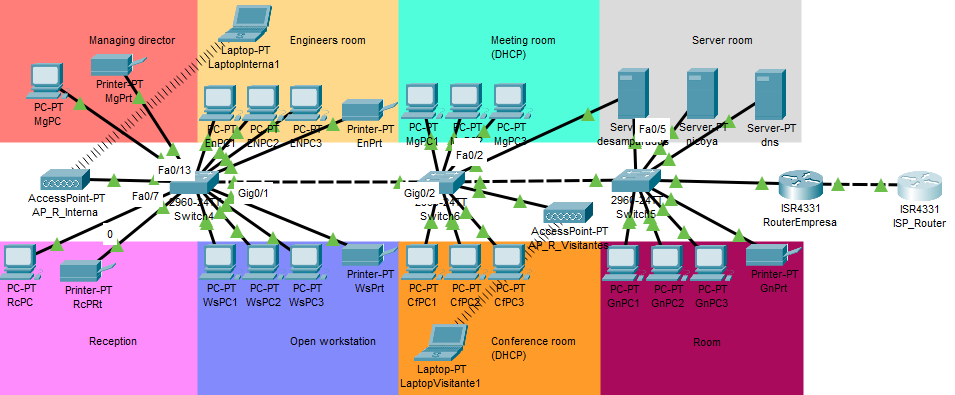
\includegraphics[width=\linewidth]{figures/simulacion.png}
        \caption{Captura de la topología de la red en la simulación}
        \label{fig: simulacion}
    \end{figure}

    \subsection{Configuración de equipo}

        Para el switch4 y switch6 se define la red local de area virtual
        para uso interno de la compañia. La configuración y
        asignación de puertos de esta se realiza con la siguiente
        lista de comandos:

        \begin{verbatim}
    en
	show vlan
	conf t
	vlan 10
	name interna
	vlan 20
	name interna
	exit
	interface range f0/1-24
	switchport mode acces
	switchport access vlan 10
	exit
	show vlan
        \end{verbatim}
    Se define el puerto troncal para ambos switches, ya que estos
    se conectan con el switch5, que gestiona la red de visitantes.

        \begin{verbatim}
    en
	conf t
	interface g0/1
	switchport mode trunk
	switchport trunk allowed vlan 10,20
	interface g0/2
	switchport mode trunk
	switchport trunk allowed vlan 10,20
	exit
	exit

        \end{verbatim}

        Para el switch5, se configura su red local de area virtual
        de la siguiente manera:

        \begin{verbatim}
    en
	show vlan
	conf t
	vlan 10
	name interna
	vlan 20
	name interna
	exit
	interface range f0/1-24
	switchport mode acces
	switchport access vlan 20
	exit
	show vlan
        \end{verbatim}

        Cabe mencionar que las redes locales de area virtual deben ser
        creadas en todos los switches para asi poder direccionar el 
        trafico de tramas correctamente en la capa de enlace a través
        de los puertos troncales. La configuración de estos puertos se 
        presenta a continuación:

        \begin{verbatim}
    en
	conf t
	interface g0/1
	switchport mode trunk
	switchport trunk allowed vlan 10,20
	interface g0/2
	switchport mode trunk
	switchport trunk allowed vlan 10,20
	exit
	exit
        \end{verbatim}

        El router se configura en la topología R.O.A.S ({\it Router
        on a Stick}), donde se secciona un puerto GigabitEthernet
        con dos direcciones IP, para las dos vlan anteriormente
        definidas. Se utiliza el protocolo dot1Q, proveniente del
        estándar IEEE 802.1Q para etiquetar las vlan, permitiendo
        así el acceso al exterior.

        \begin{verbatim}
    en
	conf t
	int gi 0/0/1.10
	encapsultaion dot1Q 10
	ip address 10.0.0.1 255.255.255.0
	exit
	int gi 0/0/1.20
	encapsulation dot1Q 20
	ip address 10.0.1.1 255.255.255.0
	exit
	int gi 0/0/1
	no shu
	exit
        \end{verbatim}

        Finalmente, se realiza la configuración de red:

        \begin{verbatim}
    en
	conf t
	router rip
	network 10.0.0.0
	network 10.0.1.0
	exit
	exit
        \end{verbatim}



    \subsection{Comportamiento Esperado}

        En la figura \ref{fig: pings} se envian mensajes entre las zonas,
        donde se logra observar que ambas partes de la red se pueden
        comunicar con el router y hacia el exterior, sin embargo esto
        no sucede para visitantes y los dispositivos internos.
    
        \begin{figure}[H]
            \begin{minipage}{\textwidth}
                 \begin{minipage}{0.47\textwidth}
                    \begin{figure}[H]
                        \centering
                        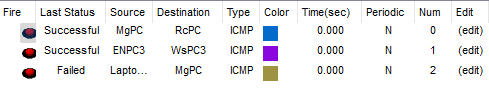
\includegraphics[width=\textwidth]{figures/firstSetPing.png}
                    \end{figure}
                 \end{minipage}\hfill
                 \begin{minipage}{0.47\textwidth}
                    \begin{figure}[H]
                        \centering
                        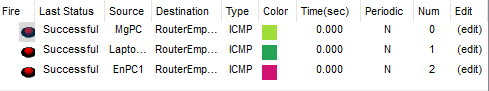
\includegraphics[width=\textwidth]{figures/secondSetPing.png}
                    \end{figure}
                 \end{minipage}
            \end{minipage}
        \caption{Mensajes Ping utilizados para comprobar el funcionamiento correcto de la topología}
        \label{fig: pings}
        \end{figure}
    
        En la figura \ref{fig: DHCP} se comprueba el funcionamiento
        correcto del servicio de la red de DHCP a través del servidor
        desamparados, el cual fue armado con dos tarjetas de red.
    
        \begin{figure}[H]
            \centering
            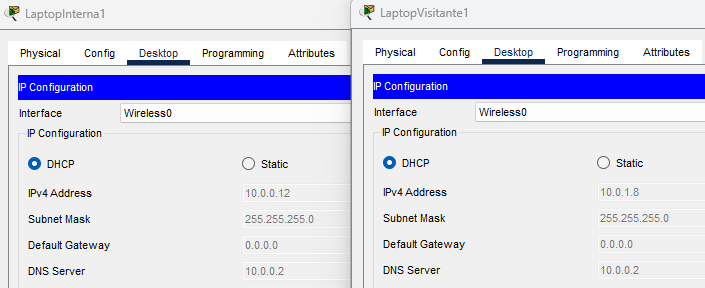
\includegraphics[width=\linewidth]{figures/DHCP3.png}
            \caption{Captura de la asignación de direcciónes IP por DHCP a laptop interna y visitante}
            \label{fig: DHCP}
        \end{figure}
    
    
\section{Presupuesto de Red}
            \lipsum[1]
